%%%%%%%%%%%%%%%%%%%%%%%%%%%%%%%%%%%%%%%%%%%%%%%%%%%%%%%%%%%%%%%%%%%
% Chapter 4: Numerical Experiment
%%%%%%%%%%%%%%%%%%%%%%%%%%%%%%%%%%%%%%%%%%%%%%%%%%%%%%%%%%%%%%%%%%%

\chapter{Numerical Experiment}
\label{chap:experiment}

\section{Dataset description}

% mô tả dữ liệu
% FX nói riêng và các chỉ số tài chính nói chung là dạng dữ liệu điển hình cho aperiodic time-series data. Do đó, chúng tôi chọn loại dữ liệu này để kiểm thử mô hình. Cụ thể, chúng tôi cấu hình hai bộ dữ liệu sử dụng dữ liệu FX. Bộ dữ liệu \verb|USD/JPY| chỉ gồm dữ liệu của cặp tiền tệ USD/JPY, được chia thành 60 tập dữ liệu con theo trình tự thời gian với kích thước bằng nhau. Dữ liệu được sample theo giờ từ năm 2000 đến năm 2024, bao gồm các thuộc tính open, low, high, và close price. Bộ dữ liệu \verb|multi-fx| bao gồm 60 cặp tiền tệ giữa 18 quốc gia Australia, Canada, Switzerland, Denmark, EU, United Kingdom, Hong Kong, Iceland, Japan, Norway, New Zealand, Singapore, Sweden, Turkey, United States, Mexico, China, South Africa. Dữ liệu có thuộc tính tương tự như \verb|USD/JPY| và được sample theo ngày từ năm 2014 đến 2024.

Foreign exchange (FX) in particular and financial indices in general are typical data types for aperiodic time-series data. Therefore, we choose this type of data to test the model. Specifically, we configure two datasets using FX data. \verb|USD/JPY| dataset consists of only data of the exchange rate between US dollar and Japanese yen. The data is sampled hourly from 2000 to 2024, including the attributes of open, low, high, and close price. \textbf{By carefully examining the transaction history as well as effectively aggregating data characteristics, we expect to forecast the movement of price without utilizing external information.}

\verb|multi-fx| dataset consists of 60 currency pairs made of 18 countries: Australia, Canada, Switzerland, Denmark, EU, United Kingdom, Hong Kong, Iceland, Japan, Norway, New Zealand, Singapore, Sweden, Turkey, United States, Mexico, China, South Africa. The data has similar attributes to \verb|USD/JPY| and sampled daily from 2014 to 2024. \textbf{By integrating analysis of multiple sources of information in the domain of FX, we expect to obtain valuable analytical insights for the indicator of interest.}

% Ngoài ra, chúng tôi sử dụng thêm 2 bộ dữ liệu: Electricity Transformer Temperature (\verb|ETT-m2|) và Weather (\verb|WTH|). Tập dữ liệu \verb|ETT-m2| bao gồm 7 trường dữ liệu, đo đạc các thông số của máy biến áp tại một tỉnh của Trung Quốc sau mỗi 15 phút trong khoảng thời gian từ July 2016 to July 2018. Tập dữ liệu \verb|WTH| bao gồm 12 trường dữ liệu, ghi nhận các thông số của thời tiết tại Weather Station of the Max Planck Biogeochemistry Institute in Jena, Germany sau mỗi 10 phút trong năm 2020. Đây là hai tập dữ liệu thể hiện tính chu kỳ rất mạnh mà \verb|NHITS| đã rất thành công trong việc dự đoán. Thực nghiệm trên chúng giúp so sánh toàn diện hơn về khả năng của phương pháp đề xuất đối với \verb|NHITS|.

In addition, we used two periodic datasets: Electricity Transformer Temperature (\verb|ETT-m2|) \cite{zhou2021informer} and Weather (\verb|WTH|) \cite{Kolle}. \verb|ETT-m2| dataset consists of 7 data fields, measuring the parameters of a transformer in a province of China every 15 minutes from July 2016 to July 2018. \verb|WTH| dataset consists of 12 data fields, recording the weather parameters at the Weather Station of the Max Planck Biogeochemistry Institute in Jena, Germany every 10 minutes in 2020. These two datasets exhibit very strong periodicity, which \verb|NHITS| has been very successful in predicting. Experiments on them provide a more comprehensive comparison of the proposed method's capabilities against \verb|NHITS|.

\section{Data pre-process}

\subsection{Temporal-ML}
\label{subsec:ml_experiment}

% viết về cách tổng hợp metric ở đây
% xét trên 1 thuộc tính cố định: chạy 60 thằng -> 60 bộ metric. lấy TBC trên 60 bộ này -> metric ± std
% chạy hết các attribute -> 4 thằng metric ± std
% -> trung bình theo kiểu mean(metric), \sqrt(mean(std^2))
Như đã đề cập trong section \ref{sec:data_prep}, để sử dụng ML, các tập dữ liệu cần phải được cấu trúc thành các task riêng biệt. Trong mỗi task, tập support chiếm 20\% dữ liệu, tập query chiếm 80\% dữ liệu. Đối với \verb|multi-fx|, mỗi cặp tiền tệ được chia thành 2 tập dữ liệu, ứng với 2 tasks. Do đó, 60 cặp tiền tệ tạo thành 120 tasks. Đối với các tập dữ liệu còn lại, mỗi tập được chia nhỏ ra thành các chuỗi thời gian, mỗi chuỗi tương ứng với một task. Trong cả quá trình, 50\% số tasks được sử dụng trong quá trình meta-training, 25\% số tasks được sử dụng trong quá trình meta-validation, số tasks còn lại được sử dụng trong meta-testing. Thống kê dữ liệu cho các task theo tập dữ liệu được trình bày trong bảng \ref{tab:stat_}.

\begin{table}
    \centering
    \caption{Statistics on datasets.}
    \label{tab:stat_}
    \begin{tblr}{
        cells = {c},
        hline{1,6} = {-}{0.08em},
        hline{2} = {-}{},
    }
    Dataset                      & Attribute & Task & Sample    & Sample/Task    \\
    \Verb|USD/JPY|               & 4         & 60   & 150,175   & 2,503          \\
    \Verb|multi-fx|              & 4         & 120   & 154,440  & 1,287          \\
    \Verb|ETT-m2|                & 7         & 48   & 69,680    & 1,452          \\
    \Verb|WTH|                   & 12        & 40   & 35,064    & 877            
    \end{tblr}
\end{table}

Vì các tập dữ liệu đều là time-series, dữ liệu trong quá trình huấn luyện không được tiết lộ bất cứ thông tin gì về tương lai. Do đó, 120 tasks của dữ liệu \verb|multi-fx| được chia như hình \ref{fig:multi_fx_split}. Đối với các tập dữ liệu còn lại, dữ liệu sử dụng trong quá trình huấn luyện, kiểm thử, kiểm tra phải đảm bảo thứ tự thời gian từ quá khứ đến tương lai.

\begin{figure}
    \centering
    \begin{subfigure}[b]{0.5\textwidth}
        \centering
        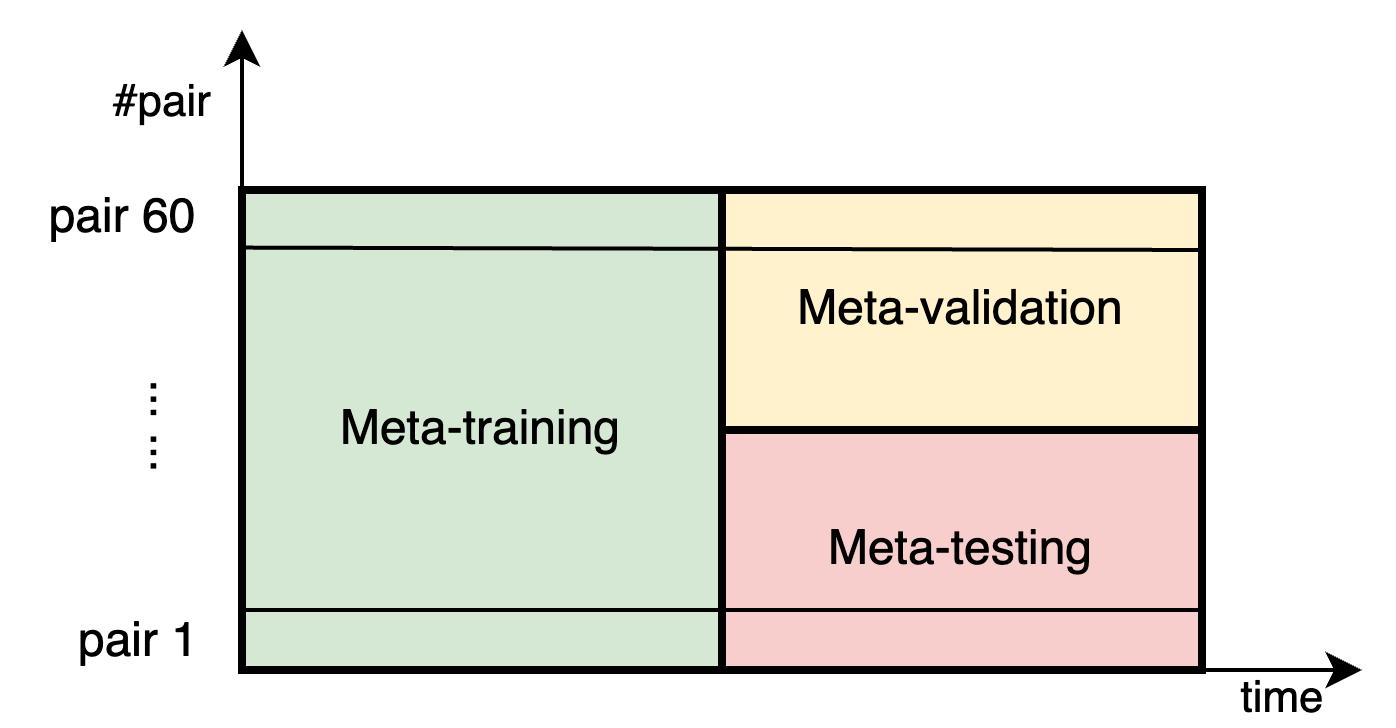
\includegraphics[width=\textwidth]{multi_fx (1).png}
        \caption{}
        \label{fig:multi_fx_split}
    \end{subfigure}%
    ~
    \begin{subfigure}[b]{0.5\textwidth}
        \centering
        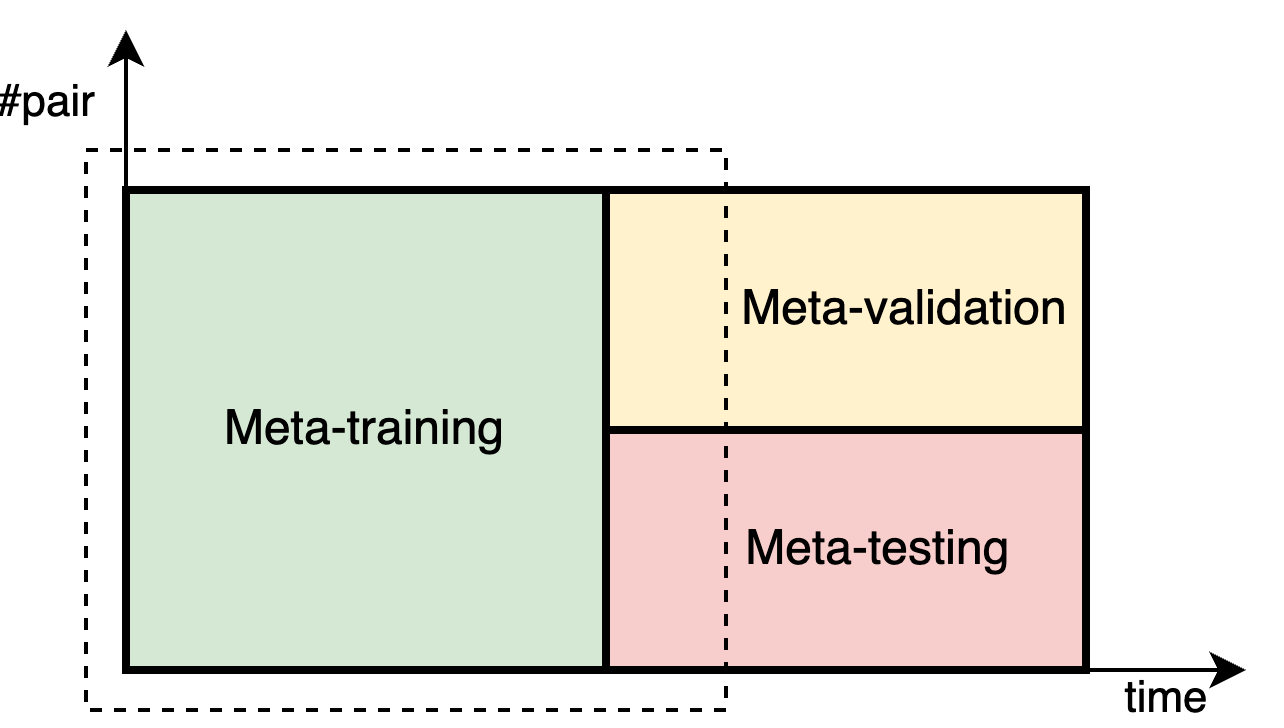
\includegraphics[width=0.92\textwidth]{multi_fx_prep.png}
        \caption{}
        \label{fig:multi_fx_prep}
    \end{subfigure}

    \cprotect\caption{(a): Splitting data for \verb|multi-fx|. (b): Pre-process for \verb|multi-fx| (dash line rectangle accounts for 20\% data of validation and testing tasks).}
    % \label{fig:ill_aperiodic}
\end{figure}

Quá trình tiền xử lý bằng \verb|z-score| theo đó được thực hiện trên toàn bộ dữ liệu huấn luyện và các tập support của dữ liệu kiểm thử và kiểm tra của từng cặp tiền tệ (see figure \ref{fig:multi_fx_prep}) vì đây là các dữ liệu đã được biết trước. Cụ thể, tiền xử lý thuộc tính $X$ được thực hiện như sau:

\begin{align}
    \mu_{X} &= \frac{1}{n} \sum_{i=1}^n{x_i} \quad \text{($n$ là số mẫu của thuộc tính $X$)} \label{eq:mean}\\
    \sigma_{X} &= \sqrt{\frac{1}{n} \sum_{i=1}^n{(x_i - \mu_X)^2}} \label{eq:std}\\
    X_{new} &= \frac{X - \mu_{X}}{\sigma_{X}} \label{eq:z_score}
\end{align}

$\mu_{X}$ và $\sigma_{X}$ thu được từ phương trình \ref{eq:mean} và \ref{eq:std} được sử dụng để chuẩn hóa cho thuộc tính $X$ trong query set của quá trình meta-validation và meta-testing.

\subsection{Baseline model}
\label{subsec:baseline_experiment}

% viết về cách tổng hợp metric ở đây
Nghiên cứu này sử dụng thuật toán \verb|NHITS| \cite{challu2023nhits} làm baseline model. \verb|NHITS| sử dụng toàn bộ thuộc tính để dự đoán xu hướng tiếp theo cho một thuộc tính trong một tập dữ liệu. Thuật toán hướng đến phân rã các giải tần và kết hợp lại để dự đoán tương lai. Đối với các tập dữ liệu \verb|USD/JPY|, \verb|ETT-m2|, và \verb|WTH|, dữ liệu tại mỗi tập được chia thành training set, validation set, và test set với tỷ lệ tương ứng 6:2:2.

Chúng tôi tiền xử lý dữ liệu huấn luyện bằng \verb|z-score| như đã đề cập ở subsection \ref{subsec:ml_experiment}. Sau đó, $\mu_{X}$ và $\sigma_{X}$ thu được từ phương trình \ref{eq:mean} và \ref{eq:std} được sử dụng để chuẩn hóa cho thuộc tính $X$ trong validation set trong quá trình tuning. Khi đã chọn được các siêu tham số tốt nhất, dữ liệu của training set và validation set được chuẩn hóa lại từ đầu, sau đó được huấn luyện với bộ siêu tham số tốt nhất để dự đoán test set.

Đối với tập dữ liệu \verb|multi-fx|, vì \verb|NHITS| không có cơ chế tổng hợp mô hình trên các tập dữ liệu khác nhau, chúng tôi lặp lại quy trình huấn luyện (huấn luyện, tuning, testing trên 60\%, 20\%, 20\% dữ liệu, respectively) cho từng cặp tiền tệ, sau đó tổng hợp metrics trên các cặp tiền tệ để thu được đánh giá cuối.

\section{Metric evaluation}

Nghiên cứu sử dụng accuracy, precision, recall, và F1 để đánh giá các mô hình:

\begin{align*}
    acc &= \frac{TP+TN}{TP+FP+TN+FN}\\
    P &= \frac{TP}{TP+FP}\\
    R &= \frac{TP}{TP+FN}\\
    F1 &= \frac{2PR}{P+R}
\end{align*}Trong đó, $TP, TN, FP, FN$ lần lượt là số mẫu \textit{true\_positive, true\_negative, false\_positive, false\_negative}.

% The study uses accuracy, precision, recall, and F1 score to evaluate the models. Accordingly, during the inference phase, the model will run on all tasks to calculate the metrics of each one. Then, the average of the metrics of the tasks is calculated to obtain the final result.

\subsection{Temporal-ML}

Giả sử thuật toán \verb|Temporal-ML| được đánh giá trên tập dữ liệu $\mathcal{D}$ gồm $a$ thuộc tính và được chia thành $n$ tasks. Quá trình đánh giá được thực hiện bằng cách để mô hình dự đoán xu hướng của từng thuộc tính với đầu vào là tất cả các thuộc tính, sau đó thực hiện hai bước tổng hợp: (1) - Tổng hợp trên task; (2) - Tổng hợp trên thuộc tính.

\textbf{Tổng hợp trên task}. Xét metric $m$ khi mô hình dự đoán thuộc tính $k$ bất kỳ ($1\leq k \leq a$). Sau khi dự đoán thuộc tính $k$, chúng ta thu được $n$ giá trị: $\{m^{(k)}_1,\dots,m^{(k)}_n\}$. Quá trình tổng hợp metrics $m$ của $n$ tasks được thực hiện như sau:

\begin{align}
    \bar{m}^{(k)} &= \frac{1}{n}\sum_{i=1}^n{m^{(k)}_i} \label{eq:mean_task}\\
    s^{(k)}_m &= \sqrt{\frac{1}{n} \sum_{i=1}^n{(m^{(k)}_i - \bar{m}^{(k)})^2}} \label{eq:std_task}
\end{align}

\textbf{Tổng hợp trên thuộc tính}. Mô hình thực hiện dự đoán tất cả $a$ thuộc tính và thu được $a$ metrics: $\left\{ \left( \bar{m}^{(k)}\pm s^{(k)}_m \right) \right\}_{k=1}^a$. Quá trình tổng hợp metric $m$ của $a$ thuộc tính diễn ra như sau:

\begin{align}
    \bar{m} &= \frac{1}{a}\sum_{k=1}^a{\bar{m}^{(k)}} \label{eq:mean_att}\\
    s_m &= \sqrt{\frac{1}{a} \sum_{k=1}^a{(s^{(k)}_m)^2}} \label{eq:std:att}
\end{align}

\subsection{Baseline model}

\verb|NHITS| cũng được đánh giá trên tập dữ liệu $\mathcal{D}$ với $a$ thuộc tính và phải thực hiện dự đoán trên từng thuộc tính. Xét metric $m$, sau quá trình dự đoán thuộc tính $k$, ta thu được $a$ giá trị: $\{m^{(k)}_1,\dots,m^{(k)}_a\}$. Quá trình tổng hợp metric $m$ của $a$ thuộc tính được thực hiện như sau:

\begin{align*}
    \bar{m} &= \frac{1}{a}\sum_{k=1}^a{m^{(k)}}\\
    s_m &= \sqrt{\frac{1}{a} \sum_{i=1}^n{(m^{(k)} - \bar{m})^2}}
\end{align*}

Như đã đề cập ở trên, \verb|NHITS| không có cơ chế tổng hợp mô hình khi kiểm thử trên dữ liệu \verb|multi-fx|. Do đó, chúng tôi kiểm thử \verb|NHITS| trên từng cặp tiền tệ trong \verb|multi-fx| và tổng hợp metrics giống như \verb|Temporal-ML|.

\subsection{Fairness in evaluation}

Gọi $m$ là số mẫu dữ liệu trong mỗi tasks, tổng số dữ liệu của quá trình huấn luyện, kiểm thử, và kiểm tra là: $mn$. Đối với \verb|NHITS|, mô hình được huấn luyện, kiểm thử, kiểm tra trên 60\%, 20\%, 20\% dữ liệu, respectively:

\begin{align*}
    \text{Train: } &0.6mn\\
    \text{Validation: } &0.2mn\\
    \text{Testing: } &0.2mn
\end{align*}

Đối với \verb|Temporal-ML|, quá trình làm giàu knowledge cho mô hình sử dụng toàn bộ dữ liệu huấn luyện và tập support của dữ liệu kiểm thử/kiểm tra. Quá trình kiểm thử/kiểm tra được thực hiện trên tập query:

\begin{align*}
    \text{Train: } &0.5mn + 20\%\left( \frac{m}{2}n \right) = 0.6mn\\
    \text{Validation: } &80\% \left( \frac{m}{2}\frac{n}{2} \right)  =0.2mn\\
    \text{Testing: } &80\% \left( \frac{m}{2}\frac{n}{2} \right) =0.2mn
\end{align*}

Do đó, với cách chia dữ liệu như trên, chúng tôi đạt được sự công bằng về số lượng mẫu dữ liệu trong quá trình kiểm thử.

\section{Hyper parameters tuning}
% quá trình fine-tune (kiểu cố định outer và quan sát inner) --> chuyển xuống phần phụ lục?

\subsection{Temporal-ML}

Trong cài đặt của chúng tôi, chúng tôi sử dụng một lớp \verb|FullyConnected| gồm 16 units với hàm kích hoạt \verb|ReLU| để biểu diễn các đặc trưng sâu hơn và rõ ràng hơn. Sau đó, đặc trưng này được truyền song song đến các hai khối \verb|BidirectionalLSTM| và \verb|CNN|. Khối \verb|BidirectionalLSTM| bao gồm 32 hidden units, các đầu ra được nối dài để tạo thành một vector cuối. Khối \verb|CNN| bao gồm hai layer \verb|CNN| có số filter lần lượt là 32 và 64. Kernel được sử dụng trong các layer có kích thước $3\times 3$. Theo sau mỗi layer \verb|CNN| là một layer \verb|MaxPooling| sử dụng kernel kích thước $2\times 2$. Kết thúc khối \verb|CNN| là một layer \verb|Flatten|. Trong trường hợp chỉ sử dụng các đặc trưng dài hạn, đầu ra của khối \verb|BidirectionalLSTM| sẽ được sử dụng để phân lớp. Nếu sử dụng thêm các đặc trưng cục bộ, đầu ra của khối \verb|BidirectionalLSTM| và \verb|CNN| sẽ được nối lại rồi truyền qua một layer phân lớp nhị phân với hàm kích hoạt \verb|Sigmoid|.

% We use a \verb|FullyConnected| layer of 16 units with a \verb|ReLU| activation function to decompose the initial feature. This feature is then passed in parallel to the \verb|BidirectionalLSTM| and \verb|CNN| blocks. The \verb|BidirectionalLSTM| block consists of 32 hidden units, the outputs of which are concatenated to form a final vector. The \verb|CNN| block consists of two \verb|CNN| layers with 32 and 64 filters, respectively. The kernel used in the layers is of size $3\times 3$. Each \verb|CNN| layer is followed by a \verb|MaxPooling| layer using a kernel of size $2\times 2$. The \verb|CNN| block ends with a \verb|Flatten| layer. Features of the \verb|BidirectionalLSTM| and \verb|CNN| blocks are then concatenated and passed through a binary classification layer with a \verb|Sigmoid| activation function.

\begin{table}[H]
    \centering
    \caption{Search space for fine-tuning our method.}
    \label{tab:our_finetune}
    \begin{tabular}{ll} 
    \toprule
    \multicolumn{1}{c}{Hyper-parameter} & \multicolumn{1}{c}{Seach space}   \\ 
    \hline
    Inner batch size (samples/batch)    & \{32\}                            \\
    Inner training step                 & \{3\}                             \\
    Outer batch size (tasks/batch)      & \{5\}                             \\
    Outer training step                 & \{100\}                           \\ 
    \hline
    Lookback window                     & \{10, 20, 30\}                    \\
    Inner learning rate                 & \{0.001, 0.005, 0.01, 0.05\}      \\
    Outer learning rate                 & \{0.001, 0.005, 0.0015, 0.0055\}  \\
    \bottomrule
    \end{tabular}
\end{table}

Quá trình fine-tune của thuật toán ML liên quan đến nhiều siêu tham số như inner batch size, outer batch size, inner training step, outer training step,... Để dễ dàng fine-tune, chúng tôi cố định hầu hết các tham số và chỉ fine-tune kích thước của lookback window, inner và outer learning rate. Chi tiết được trình bày trong bảng \ref{tab:our_finetune}.

% The fine-tuning process of ML algorithms involves many hyper-parameters such as inner batch size, outer batch size, inner training steps, outer training steps. To facilitate fine-tuning, we fix most of the parameters and only fine-tune the size of lookback window, the inner and outer learning rates. Details are presented in table \ref{tab:our_finetune}.

\subsection{Baseline model}

Đối với mô hình \verb|NHITS|, chúng tôi dựa trên \cite{challu2023nhits} để định nghĩa không gian tìm kiếm cho việc fine-tune tham số, cũng như kiến trúc mô hình. Đối với các tham số không được đề cập trong bảng, chúng tôi sử dụng giá trị mặc định của cài đặt \verb|NHITS| trong thư viện \verb|NeuralForecast| \cite{neuralforecast}. Kết quả tốt nhất của các lần fine-tune được chọn ra và báo cáo trong nghiên cứu này.

% We rely on \cite{challu2023nhits} to define the search space (table \ref{tab:nhits_finetune}) for parameter fine-tuning, as well as to fine-tune the model architecture. For parameters not mentioned in the table, we use the default values of the \verb|NHITS| implementation in the \verb|NeuralForecast| library \cite{neuralforecast}. The best results of fine-tuning process are selected and reported in this study.

\begin{table}[H]
    \centering
    \caption{Search space for fine-tuning NHITS.}
    \label{tab:nhits_finetune}
    \begin{tabular}{ll} 
    \toprule
    \multicolumn{1}{c}{Hyper-parameter} & \multicolumn{1}{c}{Seach space}                              \\ 
    \hline
    Random seed                         & \{1\}                                                        \\
    Number of stacks                    & \{3\}                                                        \\
    Number of blocks in each stack      & \{1\}                                                        \\
    Activation function                 & \{ReLU\}                                                     \\
    Batch size                          & \{256\}                                                      \\
    Epoch                               & \{500\}                                                      \\ 
    \hline
    Lookback window                     & \{5, 20, 30\}                                                \\
    Pooling kernel                      & \{{[}2,2,2], [4,4,4], [8,8,8], [8,4,1], [16,8,1]\}           \\
    Stacks' coefficients                & \{{[}168,24,1], [24,12,1], [180,60,1],[40,20,1], [64,8,1]\}  \\
    Number of MLP layers                & \{1,2\}                                                      \\
    Learning rate                       & \{0.001, 0.002, 0.005, 0.01, 0.02\}                          \\
    \bottomrule
    \end{tabular}
\end{table}
